\documentclass[a4paper, UTF8]{ctexart}
\usepackage{ctex}
\usepackage{amsmath}
\usepackage{amsthm}
\usepackage{multirow}
\usepackage{amssymb}
\usepackage{graphicx}
\usepackage{geometry}
\usepackage{bm}
\usepackage{subfigure}
\usepackage{float}
\usepackage{mathrsfs}
\renewcommand\thesection{\arabic{section}}
\newtheorem*{exercise}{\textbf{习题}}
\newtheorem*{theorem}{Theorem}
\title{Manifole Learning Homework 5}
\date{\today}
\author{安捷 1601210097}
\begin{document}
\maketitle
  \begin{exercise}[76]
    \begin{proof}
      首先,由于 $\mathbf{A}$ 是对称矩阵,因此$\mathbf{A}$有特征值分解
      \begin{equation}
        \mathbf{A} = \mathbf{U} \Lambda \mathbf{U}^T
      \end{equation}
      其中, $\Lambda$为inline首先证明题目中优化问题的解为
      \begin{equation}\label{2}
        \mathbf{X} = \mathbf{U}
        \left( \begin{array}{c}
          \max \left( \Lambda_r, 0 \right) \\
          \mathbf{0}
        \end{array} \right)
        \mathbf{U}^T
      \end{equation}
      由于
      \begin{equation}
        \lVert \mathbf{X} - \mathbf{A} \rVert_F^2 = \lVert \mathbf{X} \rVert_F^2 + \lVert \mathbf{A} \rVert_F^2 - 2 \langle \mathbf{X}, \mathbf{A}\rangle
      \end{equation}
      由von Neumann迹定理,有 $\langle \mathbf{X}, \mathbf{A} \rangle < \sum_{i=1}^N \alpha_i \beta_i$,其中, $\alpha_i, \beta_i$是 $\mathbf{X},\mathbf{A}$的奇异值的顺序和,又由于 $\mathbf{X}$ 是半正定矩阵,因此存在特征值分解
      \begin{equation}
        \mathbf{X}=\mathbf{V} \Psi \mathbf{V}^T
      \end{equation}
      其中 $\Psi$是特征值顺序排列组成的对角矩阵,所以要使得原始优化问题取得最小值,必须有 $\mathbf{U} = \mathbf{V}$,否则,无法保证 $\mathbf{X}$与$\mathbf{A}$有相同的奇异值顺序。上述论断其实有一个问题,即 $\mathbf{A}$由于不是半正定矩阵,因此其特征值的顺序与奇异值的顺序并不相同,但实际上这一问题不会影响证明的结果,由于我们后面的证明过程中会使得对应于 $\mathbf{A}$的负特征值的 $\mathbf{X}$的特征值为 $0$,因此这一问题不存在。下面考虑 $\Psi$的取值,当 $\mathbf{A}$有 $r$个非负特征值时,显然只需要使得 $\Psi$取 $\mathbf{A}$的前r个特征值即可;若 $\mathbf{A}$ 在前r个特征值会出现负特征值,此时,显然当 $\mathbf{X}$的对应特征值取为 $0$时才能保证优化问题取得最小值,上述证明过程中两步取最值得条件同时满足的情况即为\ref{2}式。同时,由于对于\ref{2}式而言,其等价于
      \begin{equation}
        \mathbf{X} = \mathbf{U_r} \Lambda_r \mathbf{U_r}^T
      \end{equation}
    \end{proof}
  \end{exercise}
  \begin{exercise}[77]
    这一问题,我尝试了四种不同的距离取法,发现Euclidean距离区分效果不显著,Angular距离和Cosine距离计算时间过长,lp距离有比较好的区分度并且计算复杂度较低,绘图如下:
    \begin{figure}[htbp!]
      \centering
      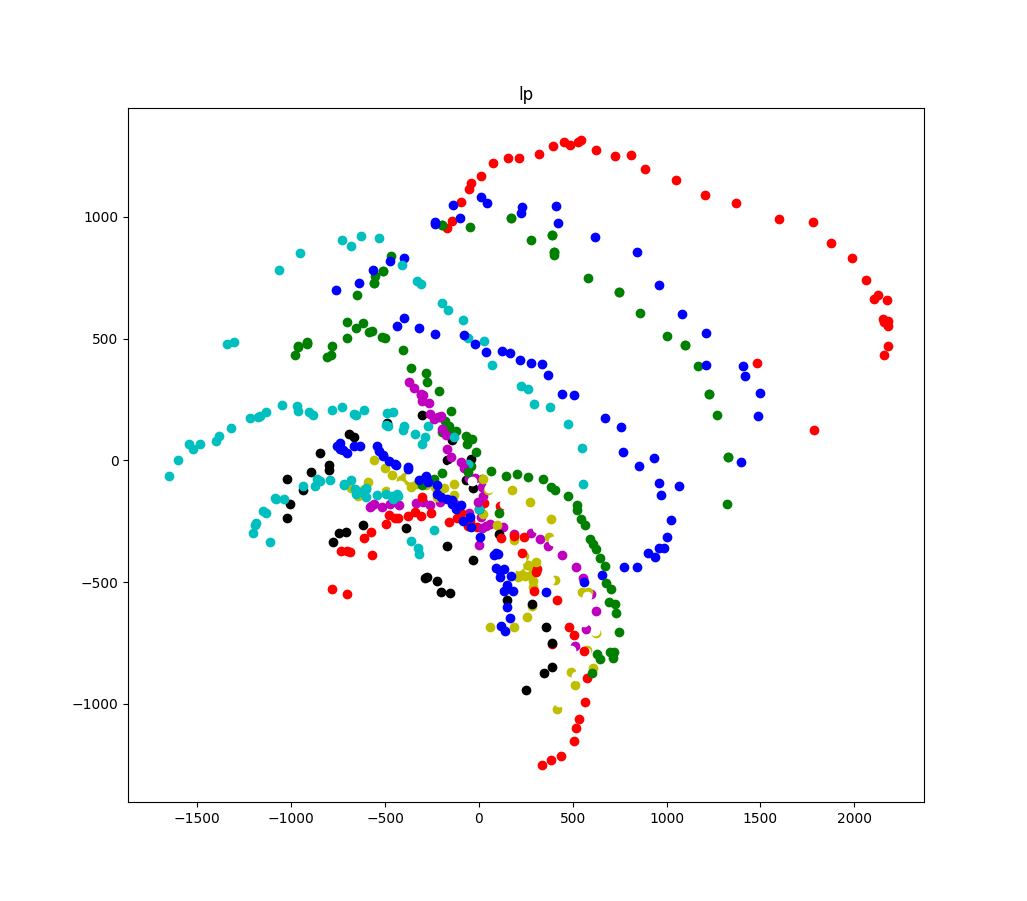
\includegraphics[width=0.8\textwidth]{fig77_1.png}
      \caption{k=2时CMDS散点图}
    \end{figure}
  \end{exercise}
  \begin{exercise}[93]
    这一道题的阈值对识别率有很大的影响,且由于随机投影矩阵的随机性,识别的准确率有很大的方差,我进行了多次的实验,在我设定的阈值情况下,平均准确率大约为80\%,每次实验的准确率情况可以运行代码。
  \end{exercise}
\end{document}
